%!TEX program = xelatex

\documentclass[10pt]{ctexart}

\usepackage{tikz}
%\usepackage{amsmath}

\begin{document}
%7.1绘图功能
%PSTricks、TikZ & pgf、METAPOST & Asymptote

%7.2TikZ绘图语言
%在导言区调用 tikz 宏包,
%就可以用以下命令和环境使用 TikZ 的绘图功能了
%\tikz[...] ⟨tikz code⟩;
%\tikz[...] {⟨tikz code 1⟩; ⟨tikz code 2⟩; ...}
%\begin{tikzpicture}[...]
%⟨tikz code 1⟩;
%⟨tikz code 2⟩;
%...
%\end{tikzpicture}
%前一种用法为 \tikz 带单条绘图命令,
%以分号结束,一般用于在文字之间插入简单的图形;
%后两种用法较为常见,使用多条绘图命令,
%可以在 figure 等浮动体中使用。

%7.2.1TikZ坐标和路径
%TikZ 用直角坐标系或者极坐标系描述点的位置。
%•直角坐标下,点的位置写作 (⟨x⟩,⟨y⟩),
%坐标 ⟨x⟩ 和 ⟨y⟩ 可以用 LATEX 支持的任意单位表示,缺省为 cm;
%• 极坐标下,点的位置写作 (⟨θ⟩:⟨r⟩)。θ 为极角,单位是度。
%我们还可以为某个点命名:
%\coordinate (A) at (⟨coordinate⟩) 
%然后就可以使用 (A) 作为点的位置了。


\begin{tikzpicture}
\draw (0,0) -- (30:1);
\draw (1,0) -- (2,1);
\coordinate (S) at (0,1);
\draw (S) -- (1,1);
\end{tikzpicture}

%坐标的表示形式还包括“垂足”形式:
\vspace{2ex}
\begin{tikzpicture}
\coordinate (S) at (2,2);
\draw[gray] (-1,2) -- (S);
\draw[gray] (2,-1) -- (S);
\draw[red] (0,0) -- (0,0 -| S);
\draw[blue] (0,0) -- (0,0 |- S);
\end{tikzpicture}

%连续使用连线时,
%可以使用 cycle 令路径回到起点,生成闭合的路径。
\vspace{2ex}
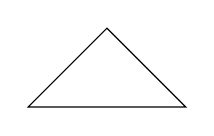
\begin{tikzpicture}
\draw (0,0) -- (1,1) -- (2,0) -- cycle;
\end{tikzpicture}

%多条路径可用于同一条画图命令中,以空格分隔:
\vspace{2ex}
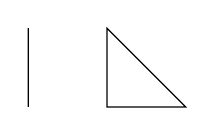
\begin{tikzpicture}
\draw (0,0) -- (0,1)
      (1,0) -- (1,1) -- (2,0) -- cycle;
\end{tikzpicture}

%矩形、圆和椭圆
\vspace{2ex}
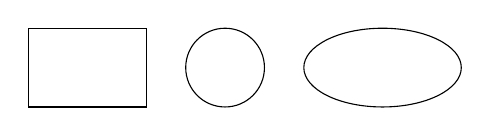
\begin{tikzpicture}
\draw (0,0) rectangle (1.5,1);
\draw (2.5,0.5) circle [radius=0.5];
\draw (4.5,0.5) ellipse [x radius=1,y radius=0.5];
\end{tikzpicture}

%直角、圆弧、椭圆弧
\vspace{2ex}
\begin{tikzpicture}
\draw (0,0) |- (1,1);
\draw (1,0) -| (2,1);
\draw (4,0) arc (0:135:1);
\draw (6,0) arc (0:135:1 and 0.5);
\end{tikzpicture}

%正弦、余弦曲线(1/4 周期
\vspace{2ex}
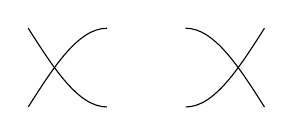
\begin{tikzpicture}
\draw (0,0) sin (1,1);
\draw (0,1) sin (1,0);
\draw (2,1) cos (3,0);
\draw (2,0) cos (3,1);
\end{tikzpicture}

%抛物线,用 bend 控制顶
\vspace{2ex}
\begin{tikzpicture}
\draw (0,0) parabola (1,2);
\draw (2,0) parabola bend (2.25,-0.25) (3,2);
\draw (4,0) parabola bend (4.75,2.25) (5,2);
\end{tikzpicture}

%二次和三次 Bézier 曲线,分别使用一个和两个控制点
\vspace{2ex}
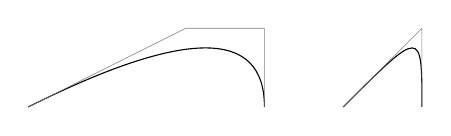
\begin{tikzpicture}
\draw (0,0) .. controls (2,1) and (3,1) .. (3,0);
\draw (4,0) .. controls (5,1) .. (5,0);
\draw[help lines] (0,0) -- (2,1) -- (3,1) -- (3,0)
(4,0) -- (5,1) -- (5,0);
\end{tikzpicture}

%网格、函数图像,网格可用 step 参数控制网格大小,
%函数图像用 domain 参数控制定义域
\vspace{2ex}
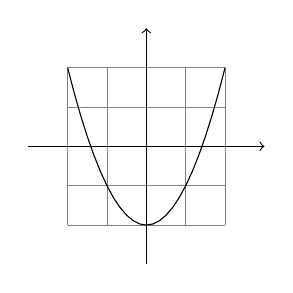
\begin{tikzpicture}
\draw[help lines,step=0.5] (-1,-1) grid (1,1);
\draw[->] (-1.5,0) -- (1.5,0);
\draw[->] (0,-1.5) -- (0,1.5);
\draw[domain=-1:1]
plot(\x,{\x*\x*2 -1});
\end{tikzpicture}

%7.2.2TikZ绘图命令和参数

%除了 \draw 命令之外,
%TikZ 还提供了 \fill 命令用来填充图形,
%\filldraw 命令则同时填充和描边。
%除了矩形、圆等现成的闭合图形外,
%\fill 和 \filldraw 命令也能够填充人为构造的闭合路径。
%\draw[...] ⟨path⟩;
%\fill[...] ⟨path⟩;
%\filldraw[...] ⟨path⟩;

%绘图参数可作为可选参数用在 tikzpiture 环境或 \tikz 命令时,
%参数会影响到所有具体的绘图命令;
%用在单个绘图命令 \draw、\filldraw 等时,只对这个命令起效。

%color/draw/fill=⟨color⟩ 为 \draw 或 \fill 等命令指定颜色。
%fill和draw分别指定填充和描边的颜色,
%而 color 同时指定,可以省略 color= 直接写颜色名称。

\vspace{2ex}
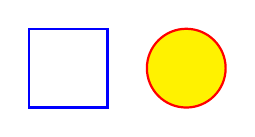
\begin{tikzpicture}[thick]
\draw[blue] (0,0) rectangle (1,1);
\filldraw[fill=yellow,draw=red] (2,0.5) circle [radius=0.5];
\end{tikzpicture}
\vspace{2ex}
%thick=⟨length⟩/thin/semithick/... 指定线条的粗细
\vspace{2ex}
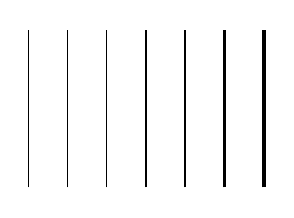
\begin{tikzpicture}
\draw[ultra thin] (0,0)--(0,2);
\draw[very thin] (0.5,0)--(0.5,2);
\draw[thin] (1,0)--(1,2);
\draw[semithick] (1.5,0)--(1.5,2);
\draw[thick] (2,0)--(2,2);
\draw[very thick] (2.5,0)--(2.5,2);
\draw[ultra thick] (3,0)--(3,2);
\end{tikzpicture}

%solid/dashed/dotted/dash dot/dash dot dot 
%指定线条类型(实线、虚线、点划线等)。
%与 dashed 对应地有 densely dashed 和 loosely dashed,
%后三种类型同理。
\vspace{2ex}
\begin{tikzpicture}
\draw[dashed] (0,0) -- (0,2);
\draw[dotted] (0.5,0) -- (0.5,2);
\draw[dash dot] (1,0) -- (1,2);
\draw[dash dot dot] (1.5,0) -- (1.5,2);
\draw[densely dotted] (2,0) -- (3,2) -- (4,0) -- cycle;
\end{tikzpicture}

%arrow⟩-⟨arrow⟩ 指定线条首尾的箭头形式。
%复杂的箭头形式需要在导言区使用 
%\usetikzlibrary {arrows.meta}。
\vspace{2ex}
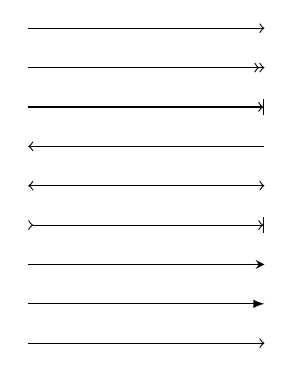
\begin{tikzpicture}
\draw[->] (0,4) -- (3,4);
\draw[->>] (0,3.5) -- (3,3.5);
\draw[->|] (0,3) -- (3,3);
\draw[<-] (0,2.5) -- (3,2.5);
\draw[<->] (0,2) -- (3,2);
\draw[>->|] (0,1.5) -- (3,1.5);
\draw[-stealth] (0,1) -- (3,1);
\draw[-latex] (0,0.5) -- (3,0.5);
\draw[-to] (0,0) -- (3,0);
\end{tikzpicture}

%rounded corners[=⟨radius⟩]/sharp corners 
%将路径转向处绘制成圆角/直角。
%可选参数⟨radius⟩ 控制圆角的半径。可以对某一段路径直接使用。
\vspace{2ex}
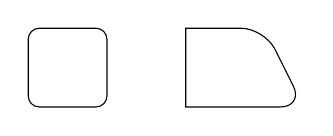
\begin{tikzpicture}
\draw[rounded corners] (0,0) rectangle (1,1);
\draw(2,0) -- (2,1) 
[rounded corners=.3cm]
-- (3,1) -- (3.5,0) 
[sharp corners] -- cycle;
\end{tikzpicture}

%scale/xshift/yshift/xslant/yslant/rotate 
%设定图形的缩放、位移和旋转\
\vspace{2ex}
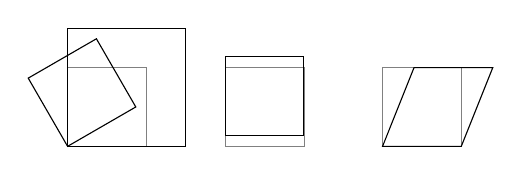
\begin{tikzpicture}
\draw[help lines](0,0) rectangle (1,1);
\draw[scale=1.5] (0,0) rectangle (1,1);
\draw[rotate=30] (0,0) rectangle (1,1);
\draw[help lines](2,0) rectangle (3,1);
\draw[yshift=4pt](2,0) rectangle (3,1);
\draw[help lines](4,0) rectangle (5,1);
\draw[xslant=0.4](4,0) rectangle (5,1);
\end{tikzpicture}

%为了重复利用绘图参数,减少代码冗余,
%TikZ 引入了“样式”的概念,可以定义一个样式包含绘图参数,
%然后将样式作为一个参数用于绘图:
\vspace{2ex}
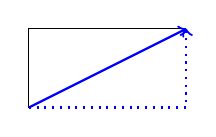
\begin{tikzpicture}
[myarrow/.style={blue,thick,->}]
\draw (0,0)--(0,1)--(2,1);
\draw[myarrow] (0,0)--(2,1);
\draw[myarrow,dotted]
(0,0)--(2,0)--(2,1); 
\end{tikzpicture}

%TikZ 还提供了 scope 环境,令绘图参数或样式在局部生效
\vspace{2ex}
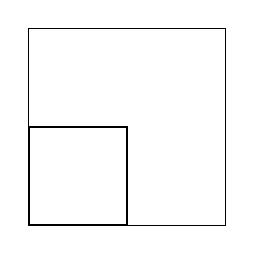
\begin{tikzpicture}
\draw (0,0) rectangle (2.5,2.5);
\begin{scope}[thick,scale=0.5]
\draw (0,0) rectangle (2.5,2.5);
\end{scope}
\end{tikzpicture}

%7.2.3TikZ文字结点
%TikZ 用 \node 命令绘制文字结点:
%\node[⟨options⟩] (⟨name⟩) at (⟨coordinate⟩) {⟨text⟩};
%(⟨name⟩) 为结点命名,
%类似 \coordinate;at (⟨coordinate⟩) 指定结点的位置。
%这两者和前面的 ⟨options⟩ 都可以省略,只有 ⟨text⟩ 是必填的。
\vspace{2ex}
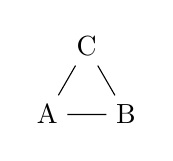
\begin{tikzpicture}
\node (A) at (0,0) {A};
\node (B) at (1,0) {B};
\node (C) at (60:1) {C};
\draw (A) -- (B) -- (C) -- (A); 
\end{tikzpicture}

%7.2.2 小节中的参数可用于 \node 命令的配置。
%除此之外,\node 还有一些特定的参数:
%•anchor=⟨position⟩ 令结点的某个角落
% ⟨position⟩ 与 ⟨coordinate⟩ 对应。
%•centered/above/below/left/right/above left/...[=⟨length⟩]
%与anchor等效的选项。可选的⟨length⟩为节点相对于⟨coordinate⟩的距离。
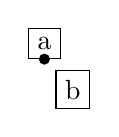
\begin{tikzpicture}
\coordinate (A) at (1,1);
\fill (A) circle[radius=2pt];
\node[draw,anchor=south] at (A) {a};
\node[draw,below right=4pt] at (A) {b};
\end{tikzpicture}

%•shape=⟨shape⟩ 结点的形状,默认可用 rectangle 和 circle,
%可省略 shape= 直接写。在
%导言区使用命令 \usetikzlibrary{shapes.geometric} 
%可用更多的形状。
%• text=⟨color⟩ 结点文字的颜色。
%• node font=⟨font command⟩ 结点文字的字体,
%形如 \bfseries 或 \itshape 等。
\vspace{2ex}
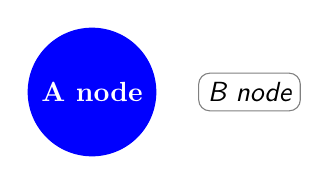
\begin{tikzpicture}
\node[circle,fill=blue,text=white,
node font={\bfseries}]
(A) at (0,0) {A node};
\node[rectangle,rounded corners,
draw=gray,
node font={\sffamily\slshape}]
(B) at (2,0) {B node};
\end{tikzpicture}

%• inner sep=⟨length⟩ / outer sep=⟨length⟩ 
%结点边界向外和向内的额外距离。
%• minimum size=⟨length⟩ / minimum height=⟨length⟩ 
%/ minimum width=⟨length⟩结点的最小大小或最小高度/宽度。

%\node 命令不仅为文字结点的位置命名,
%在 \draw 等命令中还可以使用某个结点的相对位置,
%以“东南西北”的方式命名:
\vspace{2ex}
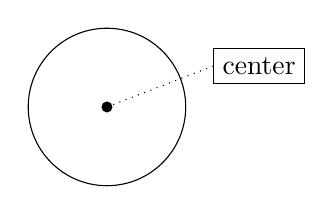
\begin{tikzpicture}
\draw (0,0) circle[radius=1];
\fill (0,0) circle[radius=2pt];
\node[draw] (P) at (15:2) {center};
\draw[dotted] (0,0) -- (P.west);
\end{tikzpicture}

%\node 命令的一种等效用法是在 
%\draw 等命令的路径中使用 node,不仅可以对某个位置标记节点,
%还能够对线标记:
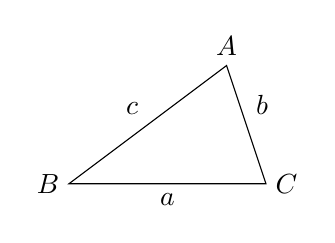
\begin{tikzpicture}
\draw (2,1.5) node[above] {$A$}
-- node[above left] {$c$}
(0,0) node[left] {$B$}
-- node[below] {$a$}
(2.5,0) node[right] {$C$}
-- node[above right] {$b$}
cycle;
\end{tikzpicture}

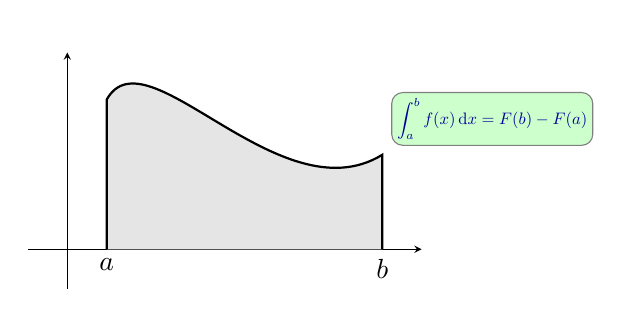
\begin{tikzpicture}
\draw[-stealth,line width=0.2pt] (-0.5,0) -- (4.5,0);
\draw[-stealth,line width=0.2pt] (0,-0.5) -- (0,2.5);
\coordinate (a) at (0.5,1.9);
\coordinate (b) at (4,1.2);
\node[below] (a0) at (a |- 0,0) {$a$};
\node[below] (b0) at (b |- 0,0) {$b$};
\filldraw[fill=gray!20,draw,thick]
(a0) -- (a) .. controls (1,2.8) and (2.7,0.4) .. (b) -- (b0) -- cycle;
\node[above right,outer sep=0.2cm, rounded corners,
fill=green!20,draw=gray,text=blue!60!black,scale=0.6]
at (b) {$\displaystyle \int_a^b {f(x)\,\mathrm{d}x} = F(b) - F(a)$};
\end{tikzpicture}

%7.2.4在TikZ中使用循环
%TikZ 通过 pgffor 功能宏包实现了简单的循环功能,语法为:
%\foreach \a in {⟨list⟩} {⟨commands⟩}
%上述语法定义了 \a 为变量,在 {⟨commands⟩} 中使用 \a 完成循环。
%⟨list⟩ 可以直接将所有值写出来,如 1,2,3,4;也可以写成省略形式,
%如 1,2,…,10。
\vspace{2ex}
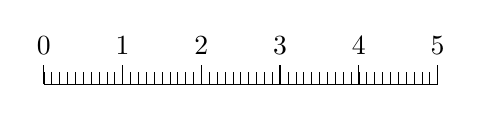
\begin{tikzpicture}
\draw (0,0)--(5,0);
\foreach \i in {0.0,0.1,...,5.0}
{\draw[very thin]
(\i,0)--(\i,0.15);}
\foreach \I in {0,1,2,3,4,5}
{\draw (\I,0)--(\I,0.25)
node[above] {\I};}
\end{tikzpicture}

%\foreach 还可使用变量对参与循环
\vspace{2ex}
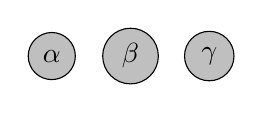
\begin{tikzpicture}
\foreach \n/\t in
{0/\alpha,1/\beta,2/\gamma}
{\node[circle,fill=lightgray,draw]
at (\n,0) {$\t$};}
\end{tikzpicture}





\end{document}